%%%%%%%%%%%%%%%%%%%%%%%%%%%%%%%%%%%%%%%%%%%%%%%%%%%%%%%%%%%%%%%%%%%%%%
% Lớp 10 | Mệnh đề. Tập hợp | Các phép toán tập hợp
% Dạng 0D1?3-3: Giao và hợp (dùng đoạn, khoảng)
% Số câu: 50  (sinh tự động bởi tach_cau.py; từ nay thầy sửa trực tiếp file này)
%%%%%%%%%%%%%%%%%%%%%%%%%%%%%%%%%%%%%%%%%%%%%%%%%%%%%%%%%%%%%%%%%%%%%%

%%%%%%%%%%%%%%%% TRẮC NGHIỆM 4 PHƯƠNG ÁN %%%%%%%%%%%%%%%%

% nguồn: MaHoaNH_TracNghiem_Lop10
\begin{ex}%[0D1N3-3]%[ma:49588746]
	Cho hai tập hợp $A=[-5;3)$,  $B=(1;+\infty)$. Khi đó $A\cap B$ là tập nào sau đây?
	\choice  { $(1;3]$}{ $[-5;+\infty)$}{\True $(1;3)$}{ $[-5;1]$}
	 \loigiai{
		$A\cap B$ là phần chung của hai tập hợp  $A\cap B=(1;3)$.
	} 
\end{ex}

% nguồn: MaHoaNH_TracNghiem_Lop10
\begin{ex}%[0D1N3-3]%[ma:e844a8e8]
	 Cho $A=(-\infty; 1]$, $B=[1;+\infty)$, $C=(0; 1]$. Khẳng định nào sau đây \textbf{sai}?
	 \choice
		{$(A \cup B) \setminus  \mathrm{C}=(-\infty; 0] \cup(1;+\infty)$}
		{\True $A \cap B \cap  \mathrm{C}=\{-1\}$}
		{$A \cup B \cup \mathrm{C}=(-\infty;+\infty)$} 
		{$(A \cap B) \setminus  \mathrm{C}=\varnothing$}
	 \loigiai{
		Ta có $A \cap B=\{1\} \Rightarrow  A \cap B \cap \mathrm{C}=\{1\}$.
	} 
\end{ex}

% nguồn: MaHoaNH_TracNghiem_Lop10
\begin{ex}%[0D1N3-3]%[ma:e863bb27]
	Cho $A=\left(-2;4\right]$, $B=\left(1;8\right)$. Tìm $A\cap  B$.
	\choice 
		 {$\left(4; 8\right)$}
		{$\left(-2;  1\right]$}
		{$\left(-2; 8\right)$} 
		 {\True $\left(1; 4\right]$}
	 \loigiai{
		 Ta có $A\cap B=\left(1; 4\right]$.
	 }
\end{ex}

% nguồn: MaHoaNH_TracNghiem_Lop10
\begin{ex}%[0D1N3-3]%[ma:3a275c96]
	Cho  tập $M=\{x \in \mathbb{R} \mid (x+3)(x-1) \geqslant 0\}$. Khi đó
	 \choice
		{$M=(-\infty;-1] \cup[3;+\infty)$} 
		{\True $M=(-\infty;-3] \cup[1;+\infty)$} 
		 {$M=[1;+\infty)$}
		 {$M=(-\infty;-3]$}
	\loigiai{ 
		Ta có $(x+3)(x-1)  \geqslant 0 \Leftrightarrow \hoac{& x \leqslant-3 \\& x \geqslant 1} $
		$\Rightarrow  M=(-\infty;-3] \cup [1;+\infty)$.
	 }
\end{ex}

% nguồn: MaHoaNH_TracNghiem_Lop10
\begin{ex}%[0D1H3-3]%[ma:76b2c2a1]
	Tổng các  số nguyên của tập $[-3;2]\setminus(1;2)$ bằng
	 \choice
		 {\True$-3$}
		 {$4$}
		 {$-5$}
		{$6$} 
	 \loigiai{
		Ta có $[-3;2]\setminus(1;2)=[3;1]\cup\{2\}$ nên chứa các số nguyên  là $-3;-2;-1;0;1;2$.\\
		Vậy tổng các số nguyên là $-3$. 
	 }
\end{ex}

% nguồn: MaHoaNH_TracNghiem_Lop10
\begin{ex}%[0D1H3-3]%[ma:33e800c6]
	Cho tập hợp $A=\left\{x\in \mathbb{R}\left\lvert\,\dfrac{2x}{x^{2}+1}\geq 1\right.\right\}$, $B$ là tập hợp tất cả các giá trị nguyên  của $b$ để phương trình $x^{2}-2bx+4=0$ vô nghiệm. Số phần tử chung của hai tập hợp trên là
	\choice 
		 {\True $1$}
		{$2$} 
		{$3$} 
		{Vô  số}
	\loigiai{ 
		Ta có $\dfrac{2x}{x^{2}+1}\geq 1\Leftrightarrow  2x\geq x^{2}+1\Leftrightarrow x^{2}-2x+1\leq 0\Leftrightarrow(x-1)^{2}\leq 0\Leftrightarrow x=1$.\\
		 Phương trình $x^{2}-2bx+4=0$ có $\Delta'=b^{2}-4$.\\
		Phương trình vô nghiệm khi và chỉ  khi $b^{2}-4<0\Leftrightarrow b^{2}<4\Leftrightarrow-2<b<2$.\\
		Có $b=1$ là  phần tử chung duy nhất của hai tập hợp.
	} 
\end{ex}

% nguồn: MaHoaNH_TracNghiem_Lop10
\begin{ex}%[0D1H3-3]%[ma:e3b41bdf]
	Cho hai tập  hợp $A=(-\infty;3]$ và $B=(1;10]$. Khi đó, tập $A\cup B$ là
	\choice 
		 {$(1;3]$}
		 {$(3;10]$}
		{\True $(-\infty;10]$} 
		{$(-\infty;1)$} 
	\loigiai{\immini{Ta  có $A\cup B=(-\infty;10]$.}
		{	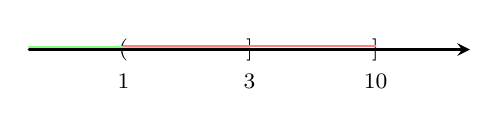
\begin{tikzpicture}[font=\footnotesize,line join=round,line cap=round,>=stealth,scale=0.8]
		\draw [line  width=1pt] [->] (-0.5,0)--(6.5,0);
		 \large
		\draw (1,0) node  {(};
		\draw (3,0) node  {]};
		\draw (5,0)  node {]};
		\normalsize 
		\draw  (1,-0.5) node {$1$};
		\draw (5,-0.5) node {$10$}; 
		\draw (3,-0.5)  node {$3$};
		\draw[color=green!50,thick] (-0.5,0.035)--(3,0.035); 
		 \draw[color=red!50,thick] (1,0.06)--(5,0.06);
	\end{tikzpicture}
		 }
	} 
\end{ex}

% nguồn: MaHoaNH_TracNghiem_Lop10
\begin{ex}%[0D1G3-3]%[ma:276d7549]
	Để phục vụ cho công việc tiêm vắc-xin  phòng chống Covid-19, Sở y tế đã huy động $30$ cán bộ đo huyết áp, $25$ cán bộ tiêm vắc-xin. Trong đó có $12$ cán bộ làm được cả $2$ công việc đo huyết áp và tiêm vắc-xin. Hỏi Sở y tế đã huy động tất cả bao nhiêu cán bộ cho công việc tiêm vắc-xin phòng chống Covid-19?
	\choice{$42$} 
		 {$31$}
		 {$55$}
		{\True  $43$}
	 \loigiai{
		Số  cán bộ được huy động là: $30+25-12=43$ cán bộ.
	 }
\end{ex}

% nguồn: MaHoaNH_TracNghiem_Lop10
\begin{ex}%[0D1B3-3]%[ma:a8c05e45]
	Lớp 10A có $51$ bạn học sinh trong đó có $31$ bạn học tiếng Anh và $27$ bạn học tiếng Nhật. Lớp 10A có bao nhiêu bạn học cả tiếng Anh và tiếng Nhật? 
	 \choice
		{\True $7$} 
		 {$9$}
		{$5$} 
		 {$12$}
	 \loigiai{
		Số học sinh học cả  tiếng Anh và tiếng Nhật của lớp 10A là $31+27-51=7$ bạn.
	 }
\end{ex}

% nguồn: MaHoaNH_TracNghiem_Lop10
\begin{ex}%[0D1K3-3]%[ma:b6032a1e]
	Một lớp học có $ 50 $ học sinh trong đó có $ 30 $ em biết chơi bóng chuyền, $ 25 $ em biết chơi bóng đá, $ 10 $ em biết chơi cả bóng đá và bóng chuyền. Hỏi có bao  nhiêu em không biết chơi môn nào trong hai môn ở trên?
	 \choice
		{$ 15  $}
		{\True$  5 $}
		{$ 20 $} 
		{$ 45 $} 
	 \loigiai{
		Gọi tập $A$ là tập học sinh biết  chơi bóng chuyền.\\Tập $B$ là tập học sinh biết chơi bóng đá.\\Khi đó số học sinh biết chơi ít nhất một trong hai môn bóng chuyền hoặc bóng đá là
		 \[|A\cup B|=30+25-10=45.\]
		Vậy số học sinh không biết chơi  môn nào là $50-45=5$.
	 }
\end{ex}

% nguồn: MaHoaNH_TracNghiem_Lop10
\begin{ex}%[0D1B3-3]%[ma:110e7aef]
	Một lớp học có $ 6 $ học sinh học giỏi môn Toán; $ 12 $ học sinh học giỏi môn Văn; $ 8 $ học sinh vừa học giỏi môn Toán và Văn; $ 19 $ học sinh  không học giỏi cả hai môn Toán và Văn. Hỏi lớp học có bao nhiêu học sinh?
	 \choice
		{\True $ 39  $}
		{$ 54  $}
		{$  31 $}
		 {$ 47 $}
	 \loigiai{
		Đáp án A đúng vì $ (16+12+19)-8=39  $.\\
		 Đáp án B sai vì học sinh tính sai $ \left[(16+12)+8\right]+19=54 $.\\
		Đáp án B sai vì học  sinh tính sai $ \left[(16-8)+(12-8)\right]+19=31 $.\\
		Đáp án B sai vì học sinh  tính sai $ 16+12+19=47 $.
	} 
\end{ex}

% nguồn: MaHoaNH_TracNghiem_Lop10
\begin{ex}%[0D1K3-3]%[ma:47c593e1]
	Lớp 10A có 10 học sinh giỏi Toán, 15 học sinh giỏi Văn, 5 học sinh giỏi cả hai môn  và 17 học sinh không giỏi môn nào. Tính số học sinh lớp 10A.
	\choice 
		 {\True $37$}
		 {$42$}
		 {$47$}
		{$32$} 
	\loigiai{ 
		\begin{itemize}
			\item  Số học sinh giỏi môn Toán hoặc môn Văn là $10+15-5=20$.
			\item Học sinh lớp 10A gồm học sinh giỏi  Toán hoặc giỏi Văn và học sinh không giỏi môn nào. Vậy số học sinh của lớp là $20+17=37$.
		\end{itemize}
	} 
\end{ex}

% nguồn: MaHoaNH_TracNghiem_Lop10
\begin{ex}%[0D1B3-3]%[ma:e929c391]
	Cho hai tập hợp $A$, $B$ có hữu hạn phần tử. Biết rằng tập hợp $B\setminus A$ có $50$ phần tử, tập hợp $A\setminus B$ có $75$ phần  tử và tập hợp $A\cap B$ có $25$ phân tử. Tính tổng số phần tử của tập hợp $A$ và $B$.
	\choice 
		 {\True $175$}
		 {$150$}
		{$75$} 
		 {$125$}
	 \loigiai{
	Trước hết ta rút ra nhận xét ba tập $A\setminus B$, $A\cap B$ và $B\setminus A$ là ba tập rời  nhau.\\
	Ta có tập $A=(A\setminus B)\cup(A\cap B)$  nên tập $A$ có $75+25=100$ phần tử.\\
	Ta có tập  $B=(B\setminus A)\cup(A\cap B)$ nên tập $A$ có $50+25=75$ phần tử.\\
	Vậy tổng số phần tử của tập $A$  và $B$ bằng $100+75=175$ phần tử.
	} 
\end{ex}

% nguồn: MaHoaNH_TracNghiem_Lop10
\begin{ex}%[0D1B3-3]%[ma:cb24451a]
	Một lớp học có $ 25 $ học sinh học khá các môn tự nhiên, $ 24 $ học sinh học khá các môn xã hội, $ 10 $ học sinh học khá cả môn tự nhiên lẫn môn xã hội, đặc biệt vẫn còn $ 3 $ học sinh chưa học khá cả hai nhóm môn ấy. Hỏi lớp có bao nhiêu học sinh chỉ khá đúng một nhóm  môn (tự nhiên hoặc xã hội).
	\choice 
		{\True $  39 $}
		{$ 26 $} 
		{$ 29  $}
		{$ 36 $} 
	 \loigiai{
		Chọn A. Số học sinh vừa khá các môn tự nhiên, vừa khá các môn xã hội chính là  số phần tử của tập hợp $ |A \cap B| $, ta có: $ |A \cup B|=|A|+|B|-|A \cap B| \Rightarrow |A|+|B|=|A \cup B|-|A \cap B| $.\\
		B. $ 26 $ (HS trừ số  lượng khá cả hai $ 2 $ lần vừa trừ thêm số lượng học sinh học khá cả $ 2 $ môn).\\
		C. $ 29 $  (HS trừ số lượng khá cả hai $ 2 $ lần).\\
		D. $ 36 $ (HS nhầm lẫn, trừ thêm số lượng $ 3 $ em chưa học khá cả $ 2 $ môn). 
	} 
\end{ex}

% nguồn: MaHoaNH_TracNghiem_Lop10
\begin{ex}%[0D1K3-3]%[ma:3d782bb3]
	Cho số  thực $a<0$. Điều kiện cần và đủ để $(-\infty;9a)\cap \left(\dfrac{4}{a};+\infty \right)\ne \varnothing $ là
	\choice 
		{\True $-\dfrac{2}{3}<a<0$} 
		 {$-\dfrac{3}{4}<a<0$}
		{$-\dfrac{2}{3}\leqslant a<0$} 
		 {$-\dfrac{3}{4}\leqslant a<0$}
	\loigiai{ 
		\[(-\infty;9a)\cap \left(\dfrac{4}{a};+\infty \right)\ne \varnothing \Leftrightarrow 9a>\dfrac{4}{a} \Leftrightarrow \left[\begin{aligned}
		&a>\dfrac{2}{3}\\ 
		 &-\dfrac{2}{3}<a<0.\\
	\end{aligned}\right.\]\\
Vì $a<0$ nên giá trị của  $a$ cần tìm là $-\dfrac{2}{3}<a<0$.}
\end{ex}

% nguồn: MaHoaNH_TracNghiem_Lop10
\begin{ex}%[0D1B3-3]%[ma:0d971846]
	Lớp $ 10A $ có $ 40 $ học sinh trong đó có $ 10 $ bạn học sinh giỏi Toán, $ 15 $ bạn  học sinh giỏi Lý, và $ 22 $ bạn không giỏi môn học nào trong hai môn Toán, Lý. Hỏi lớp $ 10A $ có bao nhiêu bạn học sinh vừa giỏi Toán vừa giỏi Lý?
	\choice 
		{\True $ 7 $} 
		{$ 25  $}
		{$  10 $}
		{$ 18 $} 
	\loigiai{ 
		Số học sinh vừa  giỏi Toán, vừa giỏi Lý chính là số phần tử của tập hợp. Từ biểu đồ Ven, ta có:\\
		$  |A \cup B|=|A|+|B|-|A \cap B| \Rightarrow |A \cap B|=|A \cup B|-|A|-|B|$.\\
		B. (HS nhầm với phép tính tổng).\\ 
		C. (HS lấy số nhỏ nhất trong hai tập hợp học sinh giỏi Toán, giỏi  Lý).\\
		D. (HS lấy sĩ số lớp trừ số bạn  không giỏi môn nào.
	 }
\end{ex}

% nguồn: MaHoaNH_TracNghiem_Lop10
\begin{ex}%[0D1B3-3]%[ma:db9fe545]
	Mỗi học sinh lớp $ 10B $ đều chơi bóng đá hoặc bóng chuyền. Biết rằng có $ 25 $ bạn chơi bóng đá, $ 20 $ bạn chơi bóng chuyền và $ 10 $ bạn  chơi cả hai môn. Hỏi lớp $ 10B $ có bao nhiêu học sinh?
	\choice 
		{\True $ 35  $}
		{$ 30 $} 
		{$  25 $}
		{$  20 $}
	 \loigiai{
		Giả sử $ A  = \text{``Học sinh chơi bóng đá''} $.\\
		$ B =  \text{``Học sinh chơi bóng chuyền''} $.\\
		$ |A \cup B| =  \text{``Học sinh chơi bóng đá hoặc bóng chuyền''} $.\\
		$  |A \cap B| = \text{``Học sinh chơi cả hai môn''} $.\\
		Số phần tử của $ |A \cup B| $  là $ 25+20-10=35 $.\\
		Số học sinh chơi  bóng đá hoặc bóng chuyền là số học sinh của lớp: $ 35 $.
	} 
\end{ex}

% nguồn: MaHoaNH_TracNghiem_Lop10
\begin{ex}%[0D1B3-3]%[ma:5c8e6a7e]
	Điểm học kỳ II môn Toán khối 10 của một nhóm  học sinh được thống kê như sau
	 \[5;5;6;6;6;7;7;8;9;9.\]
	Tìm tứ phân vị thứ  ba
	 \choice
		 {$Q_3=7$}
		{$Q_3=6{,}5$} 
		{$Q_3=6$} 
		 {\True $Q_3=8$}
	\loigiai{ 
		\begin{itemize}
			\item Sắp xếp thứ tự không giảm  mẫu số liệu ta có $5;5;6;6;6;7;7;8;9;9$.
			\item Vì cỡ mẫu là $n=10$  nên tứ phân vị thứ hai là $Q_2=\dfrac{6+7}{2}=6{,}5$.
			\item Tứ phân vị  thứ ba là trung vị của mẫu $7;7;8;9;9$. Do đó, $Q_3=8$.
		\end{itemize}
	 }
\end{ex}

% nguồn: MaHoaNH_TracNghiem_Lop10
\begin{ex}%[0D1B3-3]%[ma:26e03ce1]
	Trong số $ 45 $ học sinh của lớp $ 10A $ có $ 15 $ bạn xếp học lực giỏi, $ 20 $  bạn xếp hạnh kiểm tốt, trong đó $ 10 $ bạn vừa học lực giỏi vừa hạnh kiểm tốt. Hỏi lớp $ 10A $ có bao nhiêu bạn chưa được xếp học lực giỏi hoặc hạnh kiểm tốt?
	 \choice
		{\True $ 20 $} 
		{$  25 $}
		 {$ 15 $}
		{$ 10 $} 
	\loigiai{ 
		Giả sử $ A = \text{``Học  sinh xếp học lực giỏi''} $.\\
		$ B = \text{``Học sinh hạnh  kiểm tốt''} $.\\
		$ |A \cup B| =  \text{``Học sinh xếp học lực giỏi hoặc hạnh kiểm tốt''} $.\\
		$ |A \cap B| = \text{``Học sinh vừa học lực giỏi vừa hạnh kiểm  tốt''} $.\\
		Số phần tử của $ |A  \cup B| $ là $ 15+20-10=25 $.\\
		Số  học sinh có học lực giỏi hoặc hạnh kiểm tốt: $ 25 $.\\
		Số học sinh chưa có học lực giỏi hoặc  hạnh kiểm tốt: $ 45-25=20 $.\\
		Câu B, C, D do học  sinh tính sai đọc và hiểu chưa kỹ đề bài.
	 }
\end{ex}

% nguồn: MaHoaNH_TracNghiem_Lop10
\begin{ex}%[0D1K3-3]%[ma:4191c180]
	Gọi $A$ là tập hợp các học sinh của một lớp học có $53$ học sinh, $B$ và $C$ lần lượt là tập hợp các học  sinh thích môn Toán, tập hợp các học sinh thích môn Văn của lớp này. Biết rằng có $40$ học sinh thích môn Toán và $30$ học sinh thích môn Văn. Tìm số phần tử lớn nhất có thể có của tập hợp $B\cap C$.
	\choice 
		{$31$} 
		 {$29$}
		{\True  $30$}
		 {$32$}
	 \loigiai{
	\immini{ 
		Ta có $\heva{&n(B\cap  C)\le n(B)\\&n(B\cap C)\le n(C).}$ \\
		Suy ra $\max n(B\cap C)=\min\{n(B), n(C)\}=30$. 
		 }{
		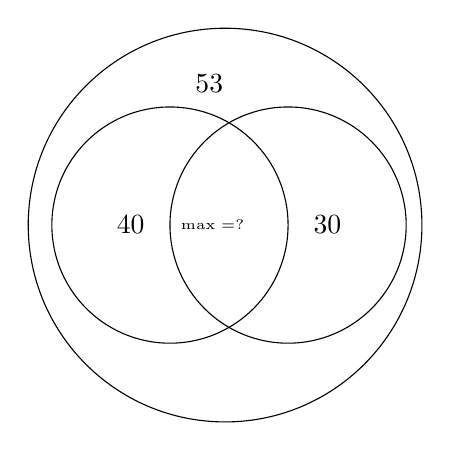
\begin{tikzpicture}
				\draw[] (0.7,0) circle (2.5cm); 
				\draw[]  (0,0) circle (1.5cm);
				\draw (1.5,0) circle  (1.5 cm);
				\draw (-0.5,0) node {$40$}; 
				\draw  (2,0) node {$30$};
				\draw (0.5,0) node  {\tiny\ $\max=?$};
				\draw (0.5,1.8) node {$53$}; 
			\end{tikzpicture}
		} 
	 }
\end{ex}

% nguồn: MaHoaNH_TracNghiem_Lop10
\begin{ex}%[0D1G3-3]%[ma:140adce8]
	Trong kì thi đánh giá năng lực lần I năm học 2018-2019 của trường THPT Triệu Quang Phục, kết quả có $86$ thí sinh đạt điểm giỏi môn Toán, $61$ thí sinh đạt điểm giỏi môn Vật lí và $76$ thí sinh đạt điểm giỏi môn Hóa học, $45$ thí sinh đạt điểm giỏi cả hai môn Toán và Vật lí, $21$ thí sinh đạt điểm giỏi cả hai môn Vật lí và Hóa học, $32$ thí sinh đạt điểm giỏi cả hai môn Toán và Hóa học, $18$ thí sinh đạt điểm giỏi cả ba môn Toán, Vật lí và Hóa học. Có $782$ thí sinh  mà cả ba môn đều không đạt điểm giỏi. Trường THPT Triệu Quang Phục có bao nhiêu thí sinh tham dự kì thi đánh giá năng lực lần I năm học 2018-2019?
	\choice 
		 {\True $925$}
		{$920$} 
		{$889$} 
		{$912$} 
	 \loigiai{
	Gọi  tập hợp học sinh giỏi môn Toán, Lí, Hóa lần lượt là $T,~L,~H$.\\
	Gọi $X$ là tập hợp thí sinh tham dự kì thi đánh giá năng lực lần I.\\ 
	Theo  đề bài ta có
	\begin{eqnarray*}
		 &n(T)=86,~n(L)=61,~n(H)=76;\\
		 &n(T\cap L)=45,~n(L\cap H)=21,~n(T\cap H)=32;\\
		&n(T\cap L\cap  H)=18.
	\end{eqnarray*}
	 Như vậy,
	\begin{eqnarray*}
		n(X)&=&782+n(T\cup L\cup H)\\ 
		&=&782+n(T)+n(L)+n(H)-(n(T\cap  L)+n(L\cap H)+n(T\cap H))+n(T\cap L\cap H)\\
		 &=&782+86+61+76-(45+21+32)+18\\
		&=&925. 
	\end{eqnarray*}
	} 
\end{ex}

% nguồn: MaHoaNH_TracNghiem_Lop10
\begin{ex}%[0D1K3-3]%[ma:8499b8b5]
	Lớp $10A$ có $17$ bạn thích chơi bóng chuyền, $22$ bạn thích chơi bóng đá. Trong số các bạn thích bóng chuyền hoặc bóng đá có $12$ bạn thích cả $2$ môn. Trong lớp vẫn còn $6$ bạn không thích bóng chuyền lẫn bóng đá. Hỏi lớp $10A$ có  bao nhiêu bạn.
	 \choice
		 {$37$}
		{\True  $33$}
		{$32$} 
		 {$35$}
	\loigiai{Ta sử dụng sơ đồ Ven để giải bài toán.\\ 
		\begin{center}
			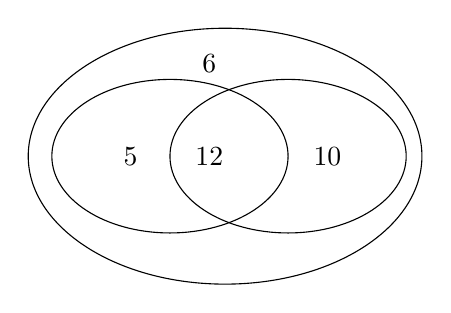
\begin{tikzpicture}[yscale=0.65]
					\draw[] (0.7,0) circle (2.5cm); 
					\draw[] (0,0) circle (1.5cm); 
					\draw (1.5,0) circle (1.5 cm); 
					\draw  (-0.5,0) node {$5$};
					\draw (2,0) node {$10$}; 
					 \draw (0.5,0) node {$12$};
					 \draw (0.5,1.8) node {$6$};
				\end{tikzpicture}
		\end{center}
		- Hình  tròn to thể hiện số học sinh cả lớp.\\
		 Như vậy, ta có:\\
		- Số bạn chỉ thích  bóng chuyền là $ 17-12=5$(bạn).\\
		- Số  bạn chỉ thích bóng đá là $22-12=10$(bạn).\\
		-  Số học sinh cả lớp là tổng các phần không giao nhau: $5+12+10+6=33$.
	} 
\end{ex}

% nguồn: MaHoaNH_TracNghiem_Lop10
\begin{ex}%[0D1B3-3]%[ma:97bd79a3]
	Trong $ 100 $ học sinh lớp $ 10 $ có $ 70 $ học sinh nói được tiếng Anh, $ 45 $ học sinh nói được tiếng Pháp và $ 23 $ học sinh nói được cả tiếng Anh và Pháp. Hỏi có bao nhiêu học sinh không nói được cả tiếng  Anh và Pháp?
	 \choice
		{\True $  8 $}
		{$  7 $}
		{$  32 $}
		 {$ 38 $}
	\loigiai{ 
	 \immini
		 {
		Ta vẽ biểu đồ Ven  như hình bên.\\
		Gọi số học sinh không nói được  cả tiếng Anh và tiếng Pháp là $ x $. Ta có:\\
		$ x+70+45-23=100  \Rightarrow x=8 $.
		 }
		{ 
		\begin{tikzpicture}[scale=.8]
				 \def\radius{2cm}
				 \coordinate (ceni);
				 \coordinate[xshift=.8*\radius] (cenii);
				\draw  (ceni) circle (\radius);
				\draw (cenii)  circle (.8*\radius);
				\draw  ([xshift=-37pt,yshift=15pt]current bounding box.north west)
					rectangle ([xshift=37pt,yshift=-30]current bounding box.south east); 
				 \node[xshift=-.6\radius] at (ceni) {$47$};
				\node[xshift=.7\radius] at (cenii)  {$22$};
				\node[xshift=.5*\radius] at (ceni)  {$23$};
				 \node[xshift=-6pt,yshift=-.6*\radius] at (ceni) {$B$};
				 \node[xshift=3pt,yshift=-.5*\radius] at (cenii) {$C$};
				\node[yshift=10pt] at (current bounding box.south) {Tổng số học sinh: $|A|=100  $};
			\end{tikzpicture}
		 }
	 }
\end{ex}

% nguồn: MaHoaNH_TracNghiem_Lop10
\begin{ex}%[0D1B3-3]%[ma:d5469948]
	Kết quả điều tra ở một lớp học cho thấy: có $ 20 $ học sinh thích bóng đá, $ 17 $ học sinh thích bơi, $ 36 $ học sinh thích chơi bóng chuyền, $  15 $ học sinh thích bóng đá và bóng chuyền, $ 10 $ học sinh thích cả ba môn, $ 12 $ không thích môn nào. Tính xem lớp học có bao nhiêu học sinh?
	 \choice
		{\True $  53 $}
		 {$ 51 $}
		 {$ 37 $}
		 {$ 56 $}
	 \loigiai{
	 \immini
		 {
		 Sử dụng sơ đồ Ven, ta có:\\
		Số học sinh của  cả lớp là:\\
		$ 20+17+36-(13+14+15)+10=53 $ (học sinh). 
		 }
		{ 
		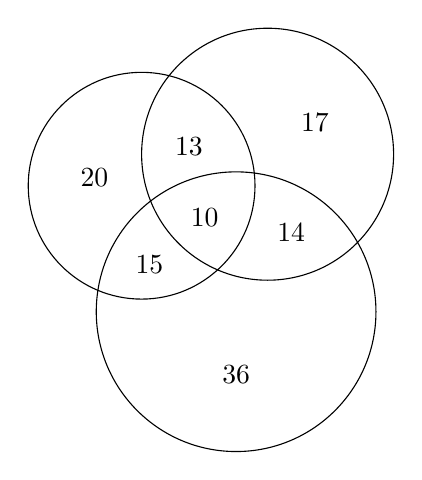
\begin{tikzpicture}[scale=.8]
				\def\radius{2cm} 
				 \coordinate (ceni);
				 \coordinate[xshift=.8*\radius,yshift=.2*\radius] (cenii);
				\coordinate[xshift=.6*\radius,yshift=-.8*\radius] (ceniii); 
				\draw (ceni)  circle (.9*\radius);
				\draw (cenii) circle (\radius); 
				 \draw (ceniii) circle (1.11*\radius);
				\node[xshift=-.3*\radius,yshift=.05*\radius] at (ceni)  {$20$};
				\node[xshift=.3*\radius,yshift=.25*\radius] at (ceni) {$13$}; 
				\node[xshift=.4*\radius,yshift=-.2*\radius] at (ceni) {$10$}; 
				 \node[xshift=.05*\radius,yshift=-.5*\radius] at (ceni) {$15$};
				\node[xshift=.15*\radius,yshift=-.5*\radius] at  (cenii) {$14$};
				\node[xshift=1.1*\radius,yshift=.4*\radius] at (ceni)  {$17$};
				\node[yshift=-.4*\radius]  at (ceniii) {$36$};
			\end{tikzpicture}
		 }
	 }
\end{ex}

% nguồn: MaHoaNH_TracNghiem_Lop10
\begin{ex}%[0D1B3-3]%[ma:5584a9c9]
	Lớp $ 10B $ có $ 7 $ học sinh giỏi Toán, $ 5 $ học sinh giỏi Lý, $ 6 $ học sinh giỏi Hóa, $ 3 $ học sinh giỏi cả Toán và Lý, $ 4 $ học sinh giỏi cả Toán và Hóa, $ 2 $ học sinh giỏi cả Lý và Hóa, $ 1 $  học sinh giỏi cả $ 3 $ môn Toán, Lý, Hóa. Số học sinh giỏi ít nhất một môn (Toán, Lý, Hóa) của lớp $ 10B $ là:
	\choice 
		 {\True $ 10 $}
		{$ 9  $}
		{$ 18  $}
		{$ 28 $} 
	\loigiai{ 
	\immini 
		{ 
		Ta  dùng biểu đồ Ven để giải:\\
		Nhìn vào biều đồ,  số học sinh giỏi ít nhất $ 1 $ trong $ 3 $ môn là:\\
		$ 1+2+1+3+1+1+1=10  $.
		 }
		 {
		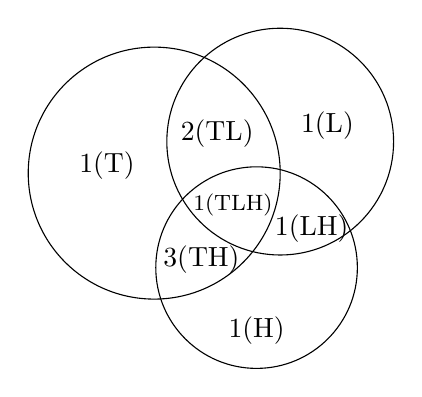
\begin{tikzpicture}[scale=.8]
				 \def\radius{2cm}
				\coordinate  (ceni);
				\coordinate[xshift=.8*\radius,yshift=.2*\radius]  (cenii);
				 \coordinate[xshift=.65*\radius,yshift=-.6*\radius] (ceniii);
				\draw (ceni) circle  (\radius);
				\draw (cenii) circle  (.9*\radius);
				\draw (ceniii) circle (.8*\radius); 
				\node[xshift=-.3*\radius,yshift=.05*\radius] at (ceni)  {$1$(T)};
				\node[xshift=.4*\radius,yshift=.25*\radius]  at (ceni) {$2$(TL)};
				\node[xshift=.3*\radius,yshift=-.55*\radius] at (ceni) {$3$(TH)}; 
				\node[xshift=.5*\radius,yshift=-.2*\radius] at (ceni) {{\footnotesize  $1$(TLH)}};
				\node[xshift=.2*\radius,yshift=-.55*\radius] at (cenii)  {$1$(LH)};
				\node[xshift=1.1*\radius,yshift=.3*\radius]  at (ceni) {$1$(L)};
				\node[yshift=-.4*\radius] at (ceniii) {$1$(H)}; 
			\end{tikzpicture}
		} 
	} 
\end{ex}

% nguồn: MaHoaNH_TracNghiem_Lop10
\begin{ex}%[0D1K3-3]%[ma:3c621817]
	Có $ 45 $ học sinh giỏi, mỗi em giỏi ít  nhất một môn. Có $ 22 $ em giỏi Văn, $ 25 $ em giỏi Toán, $ 20 $ em giỏi Anh. Có $ 8 $ em giỏi đúng hai môn Văn, Toán; có $ 7 $ em giỏi đúng hai môn Toán, Anh; có $ 6 $ em giỏi đúng hai môn Anh, Văn. Hỏi có bao nhiêu em giỏi cả ba môn Văn, Toán, Anh?
	 \choice
		{\True  $ 19 $}
		{$ 15 $} 
		{$ 14  $}
		{$ 9  $}
	 \loigiai{
	\immini 
		 {
		Theo giả thiết ta có: $ |V|=22,|T|=25, |A|=20, |V \cap T|=8,  |T \cap A|=7, |V \cap A|=6, |A \cup B \cup C|=45 $.\\
		$ |V \cup A \cup T|=|V|+|A|+|T|-|V \cap A|-|A \cap  T|-|T \cap V|+|V \cap A \cap T|\\
		\Rightarrow 45=22+20+25-6-7-8+|V \cap A \cap T|\\ 
		\Rightarrow |V \cap A  \cap T|=19 $.
		 }
		{ 
		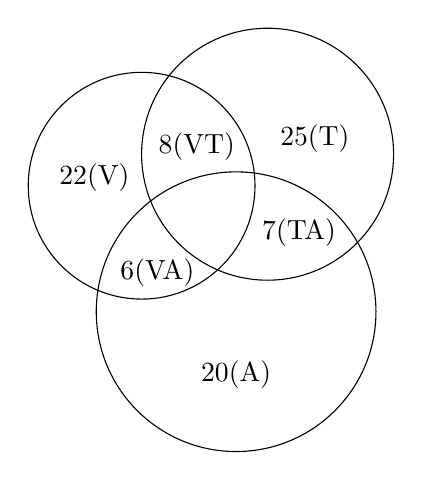
\begin{tikzpicture}[scale=.8]
				 \def\radius{2cm}
				 \coordinate (ceni);
				\coordinate[xshift=.8*\radius,yshift=.2*\radius]  (cenii);
				\coordinate[xshift=.6*\radius,yshift=-.8*\radius]  (ceniii);
				\draw  (ceni) circle (.9*\radius);
				\draw (cenii) circle (\radius); 
				\draw (ceniii)  circle (1.11*\radius);
				 \node[xshift=-.3*\radius,yshift=.05*\radius] at (ceni) {$22$(V)};
				\node[xshift=.35*\radius,yshift=.25*\radius] at (ceni)  {$8$(VT)};
				\node[xshift=.1*\radius,yshift=-.55*\radius] at  (ceni) {$6$(VA)};
				\node[xshift=.2*\radius,yshift=-.5*\radius]  at (cenii) {$7$(TA)};
				\node[xshift=1.1*\radius,yshift=.3*\radius] at (ceni)  {$25$(T)};
				\node[yshift=-.4*\radius] at  (ceniii) {$20$(A)};
			\end{tikzpicture}
		} 
	 }
\end{ex}

% nguồn: MaHoaNH_TracNghiem_Lop10
\begin{ex}%[0D1K3-3]%[ma:0849b0e6]
	Trong một lớp học có $40$ học sinh, trong đó có $30$ học sinh đạt học sinh giỏi môn Toán,  $25$ học sinh đạt học sinh giỏi môn Văn. Biết rằng chỉ có $5$ học sinh không đạt danh hiệu học sinh giỏi môn nào trong cả hai môn Toán và Văn. Hỏi có bao nhiêu học sinh chỉ học giỏi một môn trong hai môn Toán hoặc Văn?
	 \choice
		{$20$} 
		 {\True $15$}
		{$5$} 
		 {$10$}
	\loigiai{ 
		Gọi $A$  là hai tập hợp học sinh giỏi môn Toán và $B$ là hai tập hợp học sinh giỏi môn Văn.
		\begin{center}
			 {
			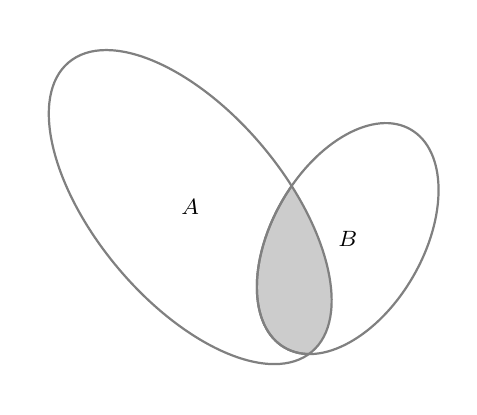
\begin{tikzpicture}[scale=.8,font=\footnotesize,line join=round,line cap=round,>=stealth]
					\def\firstcircle{(0.5cm,0)  ellipse [x radius=3cm,y radius=1.5cm,rotate=-50]}
					\def\secondcircle{(3cm,-0.5)  ellipse [x radius=2cm,y radius=1.2cm,rotate=1500]}
					 \colorlet{circle edge}{black!50}
					 \colorlet{circle area}{black!20}
					\tikzset{filled/.style={fill=circle  area,draw=circle edge,thick},
						outline/.style={draw=circle  edge,thick}}
					\begin{scope}
						\clip  \firstcircle;
						\fill[filled] \secondcircle; 
					\end{scope}
					\draw[outline] \firstcircle  node {$A$};
					\draw[outline] \secondcircle node {$B$}; 
				\end{tikzpicture}
			 }
		\end{center}
		Số học sinh  học giỏi ít nhất một môn trong hai môn Toán hoặc Văn là
		\[\left| A\cup B \right| =40-5=35, \] 
		Số học sinh học giỏi cả hai  môn Toán và Văn là
		\[\left| A\cap B  \right| =30+25-35=20, \]
		 Số học sinh chỉ học giỏi một môn trong hai môn Toán hoặc Văn là
		\[\left| (A\cup B) \backslash  (A\cap B) \right| =35-20=15. \]
	 }
\end{ex}

% nguồn: MaHoaNH_TracNghiem_Lop10
\begin{ex}%[0D1B3-3]%[ma:ff57d0e2]
	Trong Kỳ thi tốt nghiệp phổ thông, ở một trường kết quả số thí sinh đạt danh hiệu xuất sắc như sau: Về môn Toán: $ 45 $ thí sinh; về môn Vật lý: $ 36 $ thí sinh; về môn Văn: $ 43 $ thí sinh; về môn Toán hoặc môn Vật lý: $ 72 $ thí sinh; về môn Toán hoặc môn Văn: $ 74 $ thí sinh; về  môn Vật lý hoặc môn Văn: $ 65 $ thí sinh; về cả $ 3 $ môn: $ 4 $ thí sinh. Vậy có bao nhiêu học sinh nhận được danh hiệu xuất sắc về: Hai môn?
	 \choice
		{\True  $ 22 $}
		{$ 9  $}
		{$ 18  $}
		{$ 4  $}
	 \loigiai{
	\immini 
		 {
		$  |T \cap L|=45+36-72=9 $.\\
		$ |L \cap V|=43+36-65=18 $.\\ 
		$ |T \cap  V|=45+43-74=4 $.\\
		Do đó, số học sinh nhận được danh hiệu xuất sắc về $ 2 $ môn là $ 9+18+4-3\dot3=22  $.
		 }
		{ 
		\begin{tikzpicture}[scale=.8]
				 \def\radius{2cm}
				\coordinate  (ceni);
				\coordinate[xshift=.9*\radius,yshift=.1*\radius]  (cenii);
				 \coordinate[xshift=.7*\radius,yshift=-.8*\radius] (ceniii);
				\draw (ceni) circle (\radius); 
				\draw (cenii) circle  (.8*\radius);
				\draw  (ceniii) circle (.9*\radius);
				\node[xshift=-.3*\radius,yshift=.1*\radius] at (ceni)  {$45T$};
				\node[xshift=.57*\radius,yshift=-.25*\radius]  at (ceni) {$3$};
				\node[xshift=1.1*\radius,yshift=.2*\radius] at (ceni)  {$36L$};
				\node[yshift=-.3*\radius] at (ceniii)  {$43V$};
				\node[xshift=\radius,yshift=.9*\radius,right] at (ceniii) {$72 (\text{T  hoặc L})$};
				\node[xshift=\radius,yshift=.6*\radius,right] at (ceniii) {$74 (\text{T hoặc V})$}; 
				\node[xshift=\radius,yshift=.3*\radius,right] at (ceniii) {$65 (\text{V  hoặc L})$};
				\node[xshift=\radius,yshift=0*\radius,right] at (ceniii) {$3 (\text{T và  L và V})$};
			\end{tikzpicture}
		 }
	} 
\end{ex}

% nguồn: MaHoaNH_TracNghiem_Lop10
\begin{ex}%[0D1B3-3]%[ma:3c138122]
	Trong lớp $ 10C1 $ có $ 16 $ học sinh giỏi môn Toán, $ 15 $ học sinh giỏi môn Lý và $ 11 $ học sinh giỏi môn Hóa. Biết rằng có $ 9 $ học sinh vừa giỏi Toán  và Lý, $ 6 $ học sinh vừa giỏi Lý và Hóa, $ 8 $ học sinh vừa giỏi Hóa và Toán, trong đó chỉ có $ 11 $ học sinh giỏi đúng hai môn. Hỏi có bao nhiêu học sinh của lớp giỏi cả ba môn Toán, Lý, Hóa?
	 \choice
		{\True $ 4 $} 
		{$ 5 $} 
		{$ 7 $} 
		{$ 8  $}
	 \loigiai{
	 \immini
		 {
		Gọi $ T $, $ L $, $ H $ lần lượt là tập hợp các học sinh giỏi môn Toán,  Lý, Hóa. $ B $ là tập hợp học sinh giỏi đúng hai môn.\\
		 Theo giả thiết ta có: $ |T|=16,|L|=15, |H|=11, |B|=11,\\
		|T \cap L|=9, |L \cap H|=6, |H \cap T|=8  $.\\
		$  |T \cap L|+|L \cap H|+|H \cap T|-3|T \cap L \cap H|=|B|\\
		\Rightarrow |T \cap L  \cap H|=\dfrac{1}{3}\left(|T \cap L|+|L \cap H|+|H \cap T|-|B|=4\right) $.\\
		Suy ra có $ 4 $ học sinh giỏi cả ba môn Toán, Lý, Hóa. 
		 }
		 {
		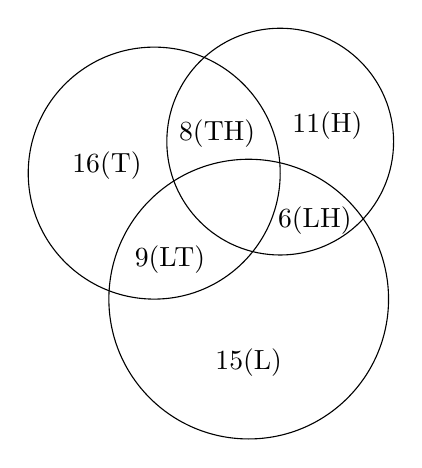
\begin{tikzpicture}[scale=.8]
				\def\radius{2cm} 
				 \coordinate (ceni);
				\coordinate[xshift=.8*\radius,yshift=.2*\radius] (cenii); 
				\coordinate[xshift=.6*\radius,yshift=-.8*\radius]  (ceniii);
				\draw (ceni)  circle (\radius);
				\draw (cenii) circle  (.9*\radius);
				\draw (ceniii) circle  (1.11*\radius);
				\node[xshift=-.3*\radius,yshift=.05*\radius]  at (ceni) {$16$(T)};
				\node[xshift=.4*\radius,yshift=.25*\radius] at (ceni) {$8$(TH)}; 
				\node[xshift=.1*\radius,yshift=-.55*\radius] at  (ceni) {$9$(LT)};
				 \node[xshift=.22*\radius,yshift=-.5*\radius] at (cenii) {$6$(LH)};
				\node[xshift=1.1*\radius,yshift=.3*\radius] at (ceni)  {$11$(H)};
				\node[yshift=-.4*\radius] at (ceniii) {$15$(L)}; 
			\end{tikzpicture}
		} 
	 }
\end{ex}

% nguồn: MaHoaNH_TracNghiem_Lop10
\begin{ex}%[0D1K3-3]%[ma:069f96de]
	Một nhóm học sinh giỏi các bộ môn:  Anh, Toán, Văn. Có $ 18 $ em giỏi Văn, $ 10 $ em giỏi Anh, $ 12 $ em giỏi Toán, $ 3 $ em giỏi Văn và Toán, $ 4 $ em giỏi Toán và Anh, $ 5 $ em giỏi Văn và Anh, $ 2 $ em giỏi cả ba môn. Hỏi nhóm đó có bao nhiêu em?
	\choice 
		{\True  $ 30 $}
		 {$ 25 $}
		{$ 20 $} 
		{$ 15  $}
	\loigiai{ 
	 \immini
		{ 
		Ký  hiệu $ A $ là tập hợp những học sinh giỏi Anh,\\
		$ T $ là tập  hợp những học sinh giỏi Toán,\\
		$ V $ là tập hợp những học  sinh giỏi Văn.\\
		Theo  giả thiết ta có: $ |V|=18, |A|=10, |T|=12, |T \cap V|=3, |T \cap A|=4, |V \cap A|=5, |A \cap B \cap C|=2 $.\\
		$ |V \cup A \cup T|=|V|+|A|+|T|-|V \cap A|-|T \cap A|-|T \cap V|+|A  \cap B \cap C|\\
		 =18+10+12-(3+4+5)+2=30 $.\\
		 Vậy nhóm đó có $ 30 $ em.
		} 
		 {
		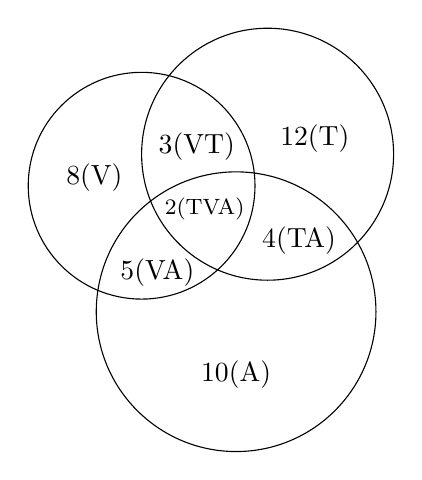
\begin{tikzpicture}[scale=.8]
				 \def\radius{2cm}
				 \coordinate (ceni);
				\coordinate[xshift=.8*\radius,yshift=.2*\radius] (cenii); 
				 \coordinate[xshift=.6*\radius,yshift=-.8*\radius] (ceniii);
				\draw (ceni)  circle (.9*\radius);
				\draw  (cenii) circle (\radius);
				\draw (ceniii)  circle (1.11*\radius);
				\node[xshift=-.3*\radius,yshift=.05*\radius] at  (ceni) {$8$(V)};
				\node[xshift=.35*\radius,yshift=.25*\radius] at (ceni)  {$3$(VT)};
				\node[xshift=.1*\radius,yshift=-.55*\radius]  at (ceni) {$5$(VA)};
				\node[xshift=.4*\radius,yshift=-.15*\radius] at (ceni) {{\footnotesize $2$(TVA)}}; 
				\node[xshift=.2*\radius,yshift=-.55*\radius] at (cenii) {$4$(TA)}; 
				\node[xshift=1.1*\radius,yshift=.3*\radius]  at (ceni) {$12$(T)};
				\node[yshift=-.4*\radius]  at (ceniii) {$10$(A)};
			\end{tikzpicture}
		 }
	 }
\end{ex}

% nguồn: MaHoaNH_TracNghiem_Lop10
\begin{ex}%[0D1B3-3]%[ma:9b3b7a23]
	Trong một khoảng thời gian nhất định, tại một  địa phương, Đài khí tượng thủy văn đã thống kê được: số ngày mưa: $ 10 $ ngày; số ngày có gió: $ 8 $ ngày; số ngày lạnh: $ 6 $ ngày; số ngày mưa và gió: $ 5 $ ngày; số ngày mưa và lạnh: $ 4 $ ngày; số ngày lạnh và có gió: $ 3 $ ngày; số ngày mưa, lạnh và có gió: $ 1 $ ngày. Vậy có bao nhiêu ngày thời tiết xấu (Có gió, mưa hay lạnh?)
	 \choice
		 {\True $ 19 $}
		{$  15 $}
		{$ 14 $} 
		{$  9 $}
	 \loigiai{
	\immini 
		 {
		Ký hiệu $ A $ là tập hợp những ngày mưa,\\ 
		 $ B $ là tập hợp những ngày có gió,\\
		$ C $ là tập hợp những  ngày lạnh.\\
		Theo  giả thiết ta có: $ |A|=10,|B|=8, |C|=6, |A \cap B|=5, |A \cap C|=4, |B \cap C|=3, |A \cap B \cap C|=1 $.\\
		 Để tìm số ngày thời thiết xấu ta sử dụng biểu đồ Ven. Ta cần tính $ |A \cup B \cup C| $
		$  |A \cup B \cup C|=|A|+|B|+|C|-|A \cap B|-|B \cap C|-|C \cap A|+|A \cap B \cap C|\\
		=10+8+6-(5+4+3)+1=13 $.\\ 
		Vậy số ngày thời tiết xấu  là $ 13 $ ngày.
		} 
		{ 
		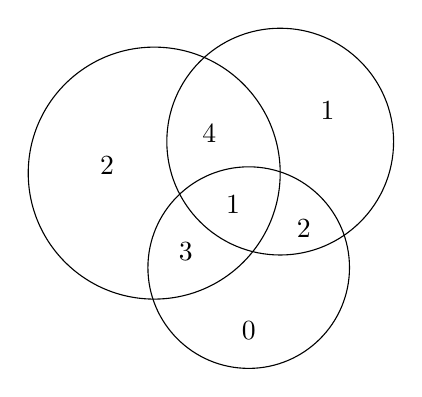
\begin{tikzpicture}[scale=.8]
				\def\radius{2cm} 
				\coordinate (ceni); 
				\coordinate[xshift=.8*\radius,yshift=.2*\radius] (cenii); 
				\coordinate[xshift=.6*\radius,yshift=-.6*\radius] (ceniii); 
				\draw (ceni)  circle (\radius);
				 \draw (cenii) circle (.9*\radius);
				\draw (ceniii)  circle (.8*\radius);
				\node[xshift=-.3*\radius,yshift=.05*\radius]  at (ceni) {$2$};
				\node[xshift=.35*\radius,yshift=.25*\radius] at (ceni)  {$4$};
				\node[xshift=.5*\radius,yshift=-.2*\radius] at (ceni) {$1$}; 
				\node[xshift=.2*\radius,yshift=-.5*\radius]  at (ceni) {$3$};
				\node[xshift=.15*\radius,yshift=-.55*\radius] at (cenii)  {$2$};
				\node[xshift=1.1*\radius,yshift=.4*\radius] at  (ceni) {$1$};
				\node[yshift=-.4*\radius] at (ceniii)  {$0$};
			\end{tikzpicture}
		} 
	 }
\end{ex}

% nguồn: MaHoaNH_TracNghiem_Lop10
\begin{ex}%[0D1K3-3]%[ma:0adc855e]
	Trong lớp $ 10C1 $ có $ 16 $ học sinh giỏi môn Toán, $ 15 $ học sinh  giỏi môn Lý và $ 11 $ học sinh giỏi môn Hóa. Biết rằng có $ 9 $ học sinh vừa giỏi Toán và Lý, $ 6 $ học sinh vừa giỏi Lý và Hóa, $ 8 $ học sinh vừa giỏi Hóa và Toán, trong đó chỉ có $ 11 $ học sinh giỏi đúng hai môn. Hỏi có bao nhiêu học sinh của lớp giỏi đúng một môn Toán, Lý hoặc Hóa?
	\choice 
		{\True $ 8 $} 
		 {$ 7 $}
		{$ 5 $} 
		 {$ 4 $}
	 \loigiai{
	 \immini
		 {
		Gọi $ T $, $ L $, $ H $ lần lượt là tập hợp các học sinh giỏi môn Toán, Lý, Hóa. $ B $ là tập hợp học  sinh giỏi đúng hai môn.\\
		Theo giả thiết ta có: $ |T|=16,|L|=15, |H|=11,  |B|=11,\\
		|T \cap L|=9, |L \cap  H|=6, |H \cap T|=8 $.\\
		Số học sinh chỉ  giỏi đúng môn Toán:\\
		$ |T|-\left(|T \cap L|+|H \cap T|-|T \cap L \cap H|\right)=16-(9+8-4)=3  $.\\
		Số  học sinh chỉ giỏi đúng môn Lý:\\
		$ |L|-\left(|T \cap L|+|L \cap H|-|T \cap L \cap  H|\right)=15-(9+6-4)=4 $.\\
		Số học  sinh chỉ giỏi đúng môn Hóa:\\
		 $ |H|-\left(|H \cap T|+|L \cap H|-|T \cap L \cap H|\right)=11-(8+6-4)=1 $.\\
		Suy ra số học sinh  giỏi đúng một môn Toán, Lý hoặc Hóa là $ 3+4+1=8 $ học sinh.
		} 
		 {
		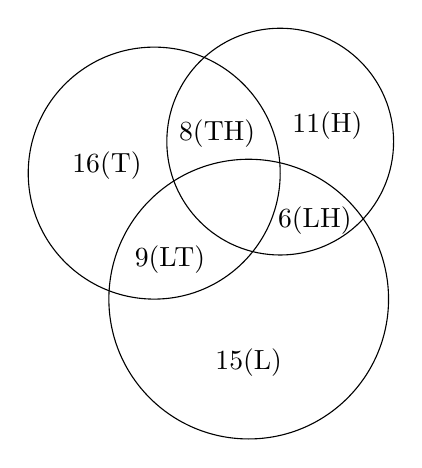
\begin{tikzpicture}[scale=.8]
				 \def\radius{2cm}
				\coordinate (ceni); 
				 \coordinate[xshift=.8*\radius,yshift=.2*\radius] (cenii);
				\coordinate[xshift=.6*\radius,yshift=-.8*\radius]  (ceniii);
				\draw  (ceni) circle (\radius);
				\draw  (cenii) circle (.9*\radius);
				\draw (ceniii)  circle (1.11*\radius);
				\node[xshift=-.3*\radius,yshift=.05*\radius] at (ceni)  {$16$(T)};
				\node[xshift=.4*\radius,yshift=.25*\radius] at  (ceni) {$8$(TH)};
				 \node[xshift=.1*\radius,yshift=-.55*\radius] at (ceni) {$9$(LT)};
				\node[xshift=.22*\radius,yshift=-.5*\radius] at  (cenii) {$6$(LH)};
				 \node[xshift=1.1*\radius,yshift=.3*\radius] at (ceni) {$11$(H)};
				\node[yshift=-.4*\radius] at  (ceniii) {$15$(L)};
			\end{tikzpicture}
		 }
	 }
\end{ex}

% nguồn: MaHoaNH_TracNghiem_Lop10
\begin{ex}%[0D1G3-3]%[ma:6044f9d1]
	Trong một khoảng thời gian nhất định, tại một địa phương, Đài khí tượng thủy văn đã thống kê được: Số ngày mưa: $10$ ngày; Số ngày có gió: $8$ ngày; Số ngày lạnh: $6$ ngày; Số ngày mưa và gió: $5$ ngày; Số ngày mưa và lạnh: $4$ ngày; Số ngày lạnh và có gió: $3$ ngày; Số ngày mưa, lạnh và có gió: $1$ ngày. Vậy có bao nhiêu ngày thời tiết xấu  (có gió, mưa hay lạnh)?
	\choice 
		{$16$} 
		 {$14$}
		 {$15$}
		{\True  $13$}
	 \loigiai{
		Ký hiệu $A$  là tập hợp những ngày mưa, $B$ là tập hợp những ngày có gió, $C$ là tập hợp những ngày lạnh.\\
		Theo giả thiết ta có $n(A)=10$, $n(B)=8$, $n(C)=6$,  $n(A\cap B)=5$, $n(A\cap C)=4$, $n(B\cap C)=3$, $n(A\cap B\cap C)=1$.\\
		Để tìm số ngày thời tiết xấu ta sử dụng biểu đồ  Ven như sau \\
		\begin{center}
			\begin{tikzpicture}[line join=round,scale=0.5]
					 \pgfmathsetmacro{\r}{2}
					\pgfmathsetmacro{\a}{\r/2} 
					 \pgfmathsetmacro{\b}{6*\r /5}
					\draw[line width=1](-\a,\b) ellipse ({\r+0.8}  and {\r+1})
						 (\a+1,\b+0.5) ellipse ({\r+0.5} and {\r+0.8})
						(\a+0.25,\b-2) ellipse ({\r+0.5}  and {\r+0.6});
					\draw (-\a-1,1.5*\r)  node{2}
						 (\a+1.5,2*\r) node{1}
						(\a,\r-3) node{6} 
						(-\a-5,\r) node{\bf (Mưa) A} 
						 (\a+5.5,1.5*\r) node{\bf (Gió) B}
						 (\a+5,\r-3) node{\bf (Lạnh) C}
						(-\a+0.5,\r-1.5) node{3} 
						 (-\a+1.5,2*\r) node{4}
						(-\a+2,\r-0.25) node{1} 
						 (-\a+3.5,\r-0.4) node{2};
				\end{tikzpicture}
		\end{center}
		Ta cần tính  $n(A\cup B\cup C)$.\\
		Xét tổng $n(A)+n(B)+n(C)$: Trong tổng này, mỗi phần tử của $A\cap B$, $B\cap C$, $C\cap A$ được tính làm hai lần nên trong tổng $n(A)+n(B)+n(C)$ ta  phải trừ đi tổng $n(A\cap B)+n(B\cap C)+n(C\cap A)$.\\
		Trong tổng $n(A)+n(B)+n(C)$ được tính  $ n(A\cap B\cap C)$ 3 lần, trong $n(A\cap B)+n(B\cap C)+n(C\cap A)$ cũng được tính $ n(A\cap B\cap C)$ 3 lần.\\ Vì vậy
		\allowdisplaybreaks 
		\begin{eqnarray*}
			n(A\cup B\cup C)&=&n(A)+n(B)+n(C)-n(A\cap B)-n(B\cap C)-n(C\cap A)+n(A\cap B\cap C)\\ 
			&=&10+8+6-(5+4+3)+1=13. 
		\end{eqnarray*}
	 Vậy số ngày thời tiết xấu là $13$ ngày.}
\end{ex}

% nguồn: MaHoaNH_TracNghiem_Lop10
\begin{ex}%[0D1B3-3]%[ma:5f619861]
	Để thành lập đội tuyển học sinh giỏi khối $ 10 $, nhà trường tổ chức thi chọn các môn Toán, Văn, Anh trên tổng số $ 111 $ học sinh. Kết quả  có: $ 70 $ học sinh giỏi Toán, $ 65 $ học sinh giỏi Văn, $ 62 $ học sinh giỏi Anh. Trong đó có $ 49 $ học sinh giỏi cả hai môn Văn và Toán, $ 32 $ học sinh giỏi cả hai môn Toán và Anh, $ 34 $ học sinh giỏi cả hai môn Văn và Anh. Xác định số học sinh giỏi cả ba môn Văn, Toán, Anh. Biết rằng có $ 6 $ học sinh không đạt yêu cầu cả ba môn.
	\choice 
		 {\True $ 23 $}
		{$  32 $}
		{$ 34  $}
		 {$ 36 $}
	 \loigiai{
	 \immini
		{ 
		Có $ 111-6=105 $ học sinh thi đạt ít nhất $ 1 $ môn.\\ 
		Gọi $ A $ là số học sinh giỏi môn  Toán và Tiếng Anh nhưng không giỏi Văn.\\
		Gọi $ B $ là số học sinh giỏi môn Toán và Văn nhưng không giỏi Tiếng Anh.\\ 
		Gọi $ C  $ là số học sinh giỏi môn Văn và Tiếng Anh nhưng không giỏi Toán.\\
		Gọi $ D $ là  số học sinh giỏi cả ba môn. Ta có hệ:\\
		$\begin{cases}
		 B+D=49\\
		A+D=32\\ 
		 C+D=34\\
		70+65+62-(A+B+C+2D)=105 
	\end{cases}\\
	\Rightarrow  92=32-D+49-D+34-D+2D\\
	\Rightarrow D=23$.\\ 
	Vậy có $  23 $ học sinh giỏi cả ba môn.
	 }
	{ 
	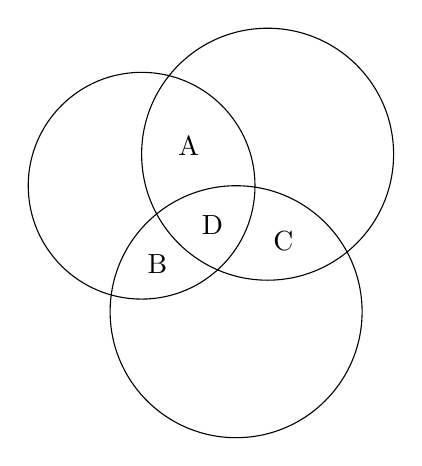
\begin{tikzpicture}[scale=.8]
			\def\radius{2cm} 
			\coordinate  (ceni);
			\coordinate[xshift=.8*\radius,yshift=.2*\radius] (cenii); 
			\coordinate[xshift=.6*\radius,yshift=-.8*\radius] (ceniii); 
			\draw (ceni)  circle (.9*\radius);
			\draw (cenii)  circle (\radius);
			\draw (ceniii)  circle (\radius);
			 \node[xshift=.3*\radius,yshift=.25*\radius] at (ceni) {A};
			\node[xshift=.1*\radius,yshift=-.5*\radius] at (ceni) {B}; 
			\node[xshift=.45*\radius,yshift=-.25*\radius] at (ceni) {D}; 
			\node[xshift=.1*\radius,yshift=-.55*\radius] at (cenii)  {C};
		\end{tikzpicture}
	} 
} 
\end{ex}

% nguồn: MaHoaNH_TracNghiem_Lop10
\begin{ex}%[0D1G3-3]%[ma:492c5f5e]
	Lớp 10B1 có $ 7$ học sinh giỏi Toán, $  5$ học sinh giỏi Lý, $ 6$ học sinh giỏi Hóa,
	$ 3$ học sinh  giỏi cả Toán và Lý, $ 4$ học sinh giỏi cả Toán và Hóa, $ 2$ học sinh giỏi cả Lý và Hóa, $ 1$ học sinh giỏi cả $ 3$ môn Toán, Lý, Hóa. Số học sinh giỏi ít nhất một môn (Toán, Lý, Hóa) của lớp 10B1 là
	 \choice
		 {\True $ 10$}
		{$28$} 
		{$18$} 
		{$9$} 
	 \loigiai{
		Ta dùng biểu đồ Ven để giải\\ 
		\begin{center}
			\begin{tikzpicture}
					\begin{scope}[line join=round,thick,fill opacity=0.4]
						 \fill[red] (0,0) circle (1.5cm);
						\fill[green] (20:2cm) circle  (1.6cm);
						 \fill[blue] (-35:1.7cm) circle (1.4cm);
					\end{scope}
					 \draw[blue] (0,0) circle (1.5cm);
					\draw[blue] (20:2cm) circle  (1.6cm);
					\draw[blue] (-35:1.7cm) circle (1.4cm); 
					\path  (-.5,0) node{$ 1 $}
						(-5:1.05) node{$ 1  $}
						(-10:2) node{$ 1 $} 
						(-55:1) node{$ 3 $} 
						(-45:2.2)  node{$ 1 $}
						(45:1.05) node{$ 2  $}
						 (25:2.5) node{$ 1 $};
					 \draw[stealth-stealth] (-65:1)--(-2,-2) node[below]{Giỏi Toán + Hóa}--(-10:.8);
					\draw[stealth-stealth] (35:1.3)--(1.1,2.5)  node[above]{Giỏi Toán + Lý}--(5:.8);
					\draw[stealth-stealth] (-10:2.4)--(4,0) node[right]{Giỏi Lý +  Hóa}--(0:1.3);
					\draw[-stealth] (-2.5,2)  node[above]{Toán}--(135:1.5);
					\draw[-stealth] (4.5,2)  node[right]{Lý}--($(20:2)+(30:1.6)$);
					 \draw[-stealth] (4.5,-2) node[right] {Hóa}--($(-35:1.7)+(-30:1.4)$);
				\end{tikzpicture}
		\end{center}
		Số học sinh giỏi Toán, Lý  mà không giỏi Hóa: $ 3-1=2$.\\
		Số học sinh giỏi Toán, Hóa  mà không giỏi Lý: $ 4-1=3$.\\
		Số học sinh giỏi Hóa, Lý mà không giỏi Toán:  $ 2-1=1$.\\
		Số  học sinh chỉ giỏi môn Lý: $ 5-2-1-1=1$.\\
		Số học sinh  chỉ giỏi môn Hóa: $ 6-3-1-1=1$.\\
		Số  học sinh chỉ giỏi môn Toán: $ 7-3-2-1=1$.\\
		Số học sinh giỏi ít nhất một (môn Toán, Lý, Hóa) là số học sinh giỏi $ 1$ môn hoặc $ 2$ môn hoặc cả $ 3$ môn: $ 1+1+1+1+2+3+1=10$. 
	 }
\end{ex}

% nguồn: MaHoaNH_TracNghiem_Lop10
\begin{ex}%[0D1K3-3]%[ma:5ed9ab51]
	Lớp $ 10B $ có $ 45  $ học sinh, trong đó có $ 25 $ em thích môn Văn, $ 20 $ em thích môn Toán, $ 18 $ em thích môn Sử, $ 6 $ em không thích môn nào, $ 5 $ em thích cả ba môn. Hỏi số em thích chỉ một trong ba môn là bao nhiêu?
	\choice 
		{\True  $ 20 $}
		{$ 30 $} 
		{$  15 $}
		 {$ 25 $}
	\loigiai{ 
	\immini 
		{ 
		Ta  vẽ biểu đồ Ven như hình bên.\\
		Gọi $ a,b,c $ theo thứ tự là số học  sinh chỉ thích môn Văn, Sử, Toán.\\
		$ x $ là số học sinh chỉ  thích hai môn là Văn và Toán.\\
		$ y  $ là số học sinh chỉ thích hai môn là Sử và Toán.\\
		$ z $ là số học sinh chỉ  thích hai môn là Văn và Sử.\\
		Ta có số em thích  nhất một môn là $ 45-6=39 $.\\
		Dựa vào sơ đồ Ven ta có phương  trình:\\
		 $(I)
		\begin{cases}
			a+x+z+5=25\\ 
			b+y+z+5=18\\ 
			c+x+y+5=20\\ 
			 x+y+z+a+b+c+5=39
		\end{cases}$
		 }
		{ 
		\begin{tikzpicture}[scale=.8]
				 \def\radius{2cm}
				 \coordinate (ceni);
				 \coordinate[xshift=.8*\radius] (cenii);
				 \coordinate[xshift=.4*\radius,yshift=-.8*\radius] (ceniii);
				\draw  (ceni) circle (.9*\radius);
				\draw (cenii)  circle (\radius);
				\draw  (ceniii) circle (1.1*\radius);
				\node[xshift=-1.05*\radius,yshift=.2*\radius] at (ceni)  {$18$(Sử)};
				\node[xshift=-.3*\radius,yshift=.2*\radius] at (ceni)  {$b$};
				\node[xshift=.35*\radius,yshift=.3*\radius] at  (ceni) {$y$};
				\node[xshift=-.1*\radius,yshift=-.45*\radius]  at (ceni) {$z$};
				\node[xshift=.35*\radius,yshift=-.25*\radius]  at (ceni) {$5$};
				\node[xshift=1.3*\radius] at (cenii) {$20$(Toán)}; 
				\node[xshift=.1*\radius,yshift=-.5*\radius]  at (cenii) {$x$};
				 \node[xshift=1.1*\radius,yshift=.2*\radius] at (ceni) {$c$};
				\node[xshift=1.3*\radius,yshift=-.2*\radius]  at (ceniii) {$25$(Văn)};
				\node[yshift=-.4*\radius] at (ceniii) {$a$}; 
			\end{tikzpicture}
		 }
		\noindent Giải hệ phương trình $ (I) $ bằng cách cộng vế với vế $  3 $ phương trình đầu ta có: $ a+b+c+2(x+y+z)+15=63 $\\
		kết hợp với phương trình cuối của hệ:  $ x+y+z+a+b+c+5=39 $ ta được:\\
		 $ a+b+c+2(39-5-a-b-c)+15=63 \Rightarrow a+b+c=20 $.\\
		Vậy chỉ có $ 20 $ em thích chỉ một môn  trong ba môn trên.
	 }
\end{ex}


%%%%%%%%%%%%%%%% ĐÚNG/SAI %%%%%%%%%%%%%%%%

% nguồn: MaHoaNH_DungSai_Lop10
\begin{ex}%[0D1N3-3]%[ma:106f526b]
	Cho các  tập hợp $A=\{x\in\mathbb{R}|x\le 3\}$, $B=\{x\in\mathbb{R}|-3<x<5\}$, $C=[3;+\infty)$
	\choiceTF 
		{\True $A\cap  B=(-3;3]$}
		{ $A\cup B=(-\infty;5]$} 
		{ $A\cap  C=\varnothing$}
		{\True $B\cup C=(-3;+\infty)$} 
	\loigiai{$A=(-\infty;3]$, $B=(-3;5)$, $C=[3;+\infty)$. 
		\begin{itemchoice}
			\itemch $A\cap B=(-3;3]$. 
			 \itemch $A\cup B=(-\infty;5)$.
			\itemch $A\cap  C=\{3\}$.
			 \itemch $B\cup C=(-3;+\infty)$.
		\end{itemchoice}
	} 
\end{ex}

% nguồn: MaHoaNH_DungSai_Lop10
\begin{ex}%[0D1N3-3]%[ma:ec035980]
	 Cho các tập hợp $A=(-2;5)$, $B=(0;+\infty)$ và $C=[5;7]$.
	\choiceTF 
		{$A\cup B=(0;5)$} 
		{\True  $B\cap C=[5;7]$}
		{  $A\cap C=\{5\}$}
		{\True  $A\cap B=(0;5)$}
	\loigiai{ 
		\begin{itemchoice}
			\itemch $A\cup B=(-2;+\infty)$. 
			 \itemch $B\cap C=[5;7]$.
			 \itemch $A\cap C=\varnothing$.
			\itemch  $A\cap B=(0;5)$.
		\end{itemchoice}
	} 
\end{ex}


%%%%%%%%%%%%%%%% TỰ LUẬN %%%%%%%%%%%%%%%%

% nguồn: MaHoaNH_TuLuan_Lop10
\begin{bt}%[0D1H3-3]%[ma:51047e99]
	Cho tập hợp  $A=\{x\in \mathbb{R}\mid-1<x\leq 5\}$ và $B=\{x\in \mathbb{R}\mid 0\leq x<7\}$. Hãy tìm tập hợp $C$ thỏa mãn
	\begin{enumEX}{2}
		\item $C=A\cup B$; 
		\item  $C=A\cap B$;
		\item $C=(A\cup B)\backslash(A\cap B)$; 
		\item  $C=(A\backslash B)\cup(B\backslash A)$;
	\end{enumEX}
	\loigiai{ 
		\begin{enumerate}
			\item Ta  có $C=A\cup B=\{x\in \mathbb{R}\mid-1<x<7\}$.
			\item Ta có $C=A\cap  B=\{x\in \mathbb{R}\mid 0\leq x\leq 5\}$.
			\item Ta có $A\cup B=\{x\in \mathbb{R}\mid-1<x<7\},A\cap B=\{x\in \mathbb{R}\mid 0\leq x\leq  5\}$.\\
			Suy ra $C=(A\cup  B)\backslash(A\cap B)=C=A\cap B=\{x\in \mathbb{R}\mid-1<x<0 \text{ hoặc }5<x<7\}$.
			\item Ta có $A\backslash B=\{x\in \mathbb{R}\mid-1<x<0\};B\backslash A=\{x\in  \mathbb{R}\mid 5<x<7\}$.\\
			Suy  ra $C=(A\backslash B)\cup(B\backslash A)=\{x\in \mathbb{R}\mid-1<x<0\text{ hoặc }5<x<7\}$.
		\end{enumerate}
	 }
\end{bt}

% nguồn: MaHoaNH_TuLuan_Lop10
\begin{bt}%[0D1H3-3]%[ma:d3c08f27]
	Chứng minh rằng 
	\begin{enumEX}{2}
		\item Nếu $A\subset B$ thì $A\cap B=A$. 
		\item Nếu $A\subset C$ và $B\subset C$ thì $A\cup  B\subset C$.
		\item Nếu $A\cup B=A\cap B$  thì $A=B$.
		\item Nếu $A\subset B$ và $A\subset C$ thì $A\subset B\cap C$. 
	\end{enumEX}
	\loigiai{ 
		\begin{enumerate}
			\item Nếu  $A\subset B$ thì $A\cap B=A$.\\
			Thật  vậy\\
			Xét với mọi $x\in A$ thì $x\in B$ (do $A\subset  B$) nên $x\in A\cap B\Rightarrow A\subset A\cap B$ (1).\\
			Hơn  nữa với mọi $x\in A\cap B\Rightarrow x\in A$ hay $A\cap B\subset A$ (2).\\
			Từ (1)  và (2), suy ra $A\cap B=A$.
			\item Xét với mọi $x\in  A\cup B\Rightarrow\hoac{&x\in A\xrightarrow{A\subset C}x\in C\\&x\in B\xrightarrow{B\subset C}x\in C}\Rightarrow x\in C\Rightarrow A\cup B\subset C$.
			\item Ta có $A\cup B=(A\backslash B)\cup(B\backslash A)\cup(A\cap B)$ mà  $A\cup B=A\cap B$ thì $A=B$ nên $\heva{&A\backslash B=\varnothing \Rightarrow A\subset B\\&B\backslash A=\varnothing \Rightarrow B\subset A}$, suy ra $A=B$.
			 \item Do $A\subset B$ và $A\subset C$ nên với mọi $x\in A\Rightarrow\heva{&x\in B\\&x\in C}\Rightarrow x\in B\cap C\Rightarrow A\subset(B\cap C)$.
		\end{enumerate}
	} 
\end{bt}

% nguồn: MaHoaNH_TuLuan_Lop10
\begin{bt}%[0D1H3-3]%[ma:bfa9c44e]
	Xác định các tập hợp sau và biểu  diễn chúng trên trục số.
	\begin{enumEX}{3}
		\item $(-4;1]\cap[0;3)$; 
		\item  $(0;2]\cup(-3;1]$;
		 \item $(-2;1)\cap(-\infty;1]$;
	\end{enumEX}
	 \loigiai{
		\begin{enumerate}
			\item  $(-4;1]\cap[0;3)=[0;1]$.
			\begin{center}
				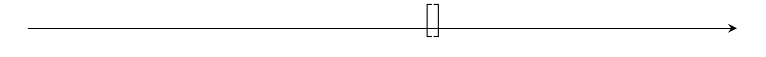
\begin{tikzpicture}[scale=1,font=\footnotesize,line join=round,line cap=round,>=stealth]
						 \draw[->](-5,0)->(4,0);
						\IntervalLR{-5}{0}; 
						\IntervalGRF{}{}{\big[}{0}; 
						 \IntervalLR{1}{4};
						\IntervalGRF{\big]}{1}{}{}; 
					\end{tikzpicture}
			\end{center}
			\item  $(0;2]\cup(-3;1]=(-3;2]$.
			\begin{center}
				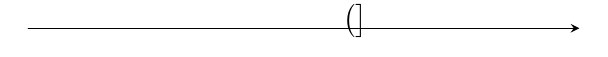
\begin{tikzpicture}[scale=1,font=\footnotesize,line join=round,line cap=round,>=stealth]
						 \draw[->](-4,0)->(3,0);
						\IntervalLR{-4}{-3}; 
						\IntervalGRF{}{}{\big (}{-3}; 
						\IntervalLR{2}{3}; 
						\IntervalGRF{\big]}{2}{}{}; 
					\end{tikzpicture}
			\end{center}
			\item  $(-2;1)\cap(-\infty;1]=(-2;1)$.
			\begin{center}
				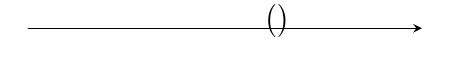
\begin{tikzpicture}[scale=1,font=\footnotesize,line join=round,line cap=round,>=stealth]
						\draw[->](-3,0)->(2,0); 
						 \IntervalLR{-3}{-2};
						 \IntervalGRF{}{}{\big (}{-2};
						\IntervalLR{1}{2}; 
						 \IntervalGRF{\big)}{1}{}{};
					\end{tikzpicture}
			\end{center}
		\end{enumerate}
	 }
\end{bt}

% nguồn: MaHoaNH_TuLuan_Lop10
\begin{bt}%[0D1V3-3]%[ma:41583045]
	Cho ba tập hợp khác rỗng $A=(2 m-1; 3-m], B=(-7; 5)$ và $C=[4; 7)$. Biết tập hợp các giá trị thực của tham  số $m$ để $A \subset B$ và $A \cap C=\varnothing$ là khoảng $(a; b)$. Tìm giá trị $3 b+a$.
	 \loigiai{
		$A \neq \varnothing \Leftrightarrow(2 m-1; 3-m] \neq \varnothing  \Leftrightarrow 2 m-1<3-m \Leftrightarrow m<\dfrac{4}{3}$.\\
		$A \subset B \Leftrightarrow(2 m-1; 3-m] \subset(-7; 5) \Leftrightarrow\heva{&-7 \leq 2  m-1 \\ &3-m<5} \Leftrightarrow\heva{&m \geq-3 \\ &m>-2} \Leftrightarrow m>-2$.\\
		$A \cap C=\varnothing \Leftrightarrow(2 m-1; 3-m] \cap[4; 7)=\varnothing \Leftrightarrow\heva{&3-m<4 \\ &7 \leq 2  m-1} \Leftrightarrow\heva{&m>-1 \\ &m \geq 4} \Leftrightarrow m>-1$.\\
		Để $A \neq \varnothing, A \subset B$ và $A \cap C=\varnothing$ thì $\heva{&m<\dfrac{4}{3}  \\ &m>-2\\&m>-1}\Leftrightarrow-1<m<\dfrac{4}{3} $.
	} 
\end{bt}

% nguồn: MaHoaNH_TuLuan_Lop10
\begin{bt}%[0D1V3-3]%[ma:552631c3]
	Cho tập hợp $A=(0;+\infty)$ và $B=\left\{x \in  \mathbb{R} \mid m x^2-6 x+m-8=0\right\}$, $m$ là tham số. Xác định $m$, biết rằng tập $B$ có đúng hai tập con và $B \subset A$.
	 \loigiai{
		Vì tập $B$ có đúng hai tập con nên $B$ có  đúng $1$ phần tử. Do đó phương trình $m x^2-6x+m-8=0$ có duy nhất một nghiệm.
		\begin{enumerate}[TH1.]
			\item  $m=0$ thì $x=-\dfrac{4}{3}
			 \Rightarrow B=\left\{-\dfrac{4}{3}\right\} \not\subset A$.
			\item $m \neq 0$ thì phương  trình có nghiệm duy nhất\\
			$\Leftrightarrow \Delta'=0$ 
			 $\Leftrightarrow 9-m(m-8)=0$
			$\Leftrightarrow-m^2+8  m+9=0$
			$\Leftrightarrow \hoac{&  m=-1 \\& m=9.}$
			\begin{itemize}
				\item Với $m=-1 \Rightarrow B=\{-3\} \not\subset A$. 
				\item Với  $m=9 \Rightarrow B=\left\{\dfrac{1}{3}\right\} \subset A$.
			\end{itemize}
			Kết hợp với điều kiện $B \subset  A$ ta có $m=9$.
		\end{enumerate}
	} 
\end{bt}

% nguồn: MaHoaNH_TuLuan_Lop10
\begin{bt}%[0D1B3-3]%[ma:22fcc953]
	Một lớp học có $ 50 $ học sinh trong đó có $ 30 $ em biết chơi bóng chuyền, $25$ em biết chơi bóng đá, $ 10 $ em biết  chơi cả bóng đá và bóng chuyền. Hỏi có bao nhiêu em không biết chơi môn nào trong hai môn ở trên?
	 \loigiai{
		Gọi tập $A$ là tập hợp các  học sinh biết chơi bóng chuyền.
		\\Tập $B$ là tập hợp các học sinh biết  chơi bóng đá.
		\\Khi đó số học sinh biết chơi ít nhất một trong hai môn bóng  chuyền hoặc bóng đá là
		$$|A\cup B|=|A|+|B|-|A\cap  B|=30+25-10=45.$$
		Vậy số học sinh không biết chơi môn nào  là $50-45=5$.
	 }
\end{bt}

% nguồn: MaHoaNH_TuLuan_Lop10
\begin{bt}%[0D1K3-3]%[ma:514190bc]
	Một lớp có $20$ bạn học giỏi Toán, $15$ bạn học giỏi Văn; trong đó có $10$ bạn giỏi cả hai môn Toán và Văn. Trong lớp còn lại $8$ bạn không học giỏi môn Toán và cũng  không học giỏi môn Văn. Vẽ biểu đồ và tính số học sinh của lớp.
	 \loigiai{
		Biểu  đồ Ven.
		\begin{center}
			\begin{tikzpicture}
					 \tkzDefPoints{-2/0/A,6/0/B,6/3/C,-2/3/D,3/1.5/E,5/1.5/F}
					 \draw (A) -- (B) -- (C) -- (D) -- (A);
					\draw (E) arc (0: -360: 2cm and 1cm); 
					\draw (F) arc  (0: -360: 2cm and 1cm);
					 \draw (0.2,1.5) node{$A$};
					\draw  (4,1.5) node{$B$};
					\draw (2,1.5)  node{$A \cap B$};
					\draw (-1.5,2)  node{$C$};
				\end{tikzpicture}
		\end{center}
		Gọi $A$ là tập  hợp các bạn giỏi Toán của lớp.\\
		 $B$ là tập hợp các bạn giỏi Văn của lớp.\\
		$C$ là tập hợp các bạn không  giỏi Toán và Văn.\\
		 $X$ là tập hợp tất cả học sinh trong lớp.\\
		Ta có $X=(A \cup  B \cup C) \setminus (A \cap B)$.\\
	Số học sinh của lớp là  $20+15+8-10=33$. }
\end{bt}

% nguồn: MaHoaNH_TuLuan_Lop10
\begin{bt}%[0D1B3-3]%[ma:6cbf187e]
	Lớp $10A$ có $15$ bạn thích môn Văn, $20$ bạn thích môn Toán. Trong số  các bạn thích văn hoặc toán có $8$ bạn thích cả $2$ môn. Trong lớp vẫn còn $10$ bạn không thích môn nào trong $2$ môn Văn và Toán. Hỏi lớp $10A$ có bao nhiêu học sinh?
	\loigiai{Ta sử dụng sơ đồ Ven. 
		\begin{center}
			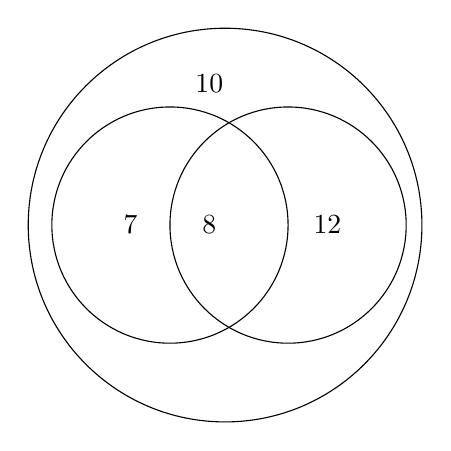
\begin{tikzpicture}
					\draw[] (0.7,0)  circle (2.5cm);
					 \draw[] (0,0) circle (1.5cm);
					\draw (1.5,0)  circle (1.5 cm);
					 \draw (-0.5,0) node {$7$};
					\draw (2,0) node  {$12$};
					\draw (0.5,0)  node {$8$};
					 \draw (0.5,1.8) node {$10$};
				\end{tikzpicture}
		\end{center}
		\begin{itemize}
			 \item Hình tròn lớn ngoài cùng thể hiện số học sinh cả lớp.\\
			Như vậy, ta  có:\\
			\item Số bạn chỉ thích Văn là  $ 15-8=7$(bạn).\\
			\item  Số bạn chỉ thích Toán là $20-8=12$(bạn).\\
			\item Số học sinh cả  lớp là tổng các phần không giao nhau: $7+8+12+10=37$.
		\end{itemize}
	} 
\end{bt}

% nguồn: MaHoaNH_TuLuan_Lop10
\begin{bt}%[0D1B3-3]%[ma:4b106b78]
	Trong kì thi học sinh giỏi cấp trường, lớp 10C1 có $45$ học sinh trong đó có $17$ bạn đạt học sinh giỏi Văn, $25$ bạn đạt học sinh giỏi Toán và $13$ bạn học sinh không đạt học sinh giỏi. Tìm số học sinh giỏi cả Văn và Toán  của lớp 10C1.
	\loigiai{ 
	\immini{ 
		\begin{itemize}
			\item Gọi $A$, $B$ theo thứ tự  là tập hợp các học sinh giỏi Văn và giỏi Toán của lớp.
			Theo đề ta có $|A|=17$,  $|B|=25$, $|A\cup B|= 45-13=32$.
			\item Số học  sinh giỏi cả Văn và Toán là $$|A \cap B |=|A| + |B| - |A \cup B|=25+17-32=10.$$
		\end{itemize}
		 }
		{	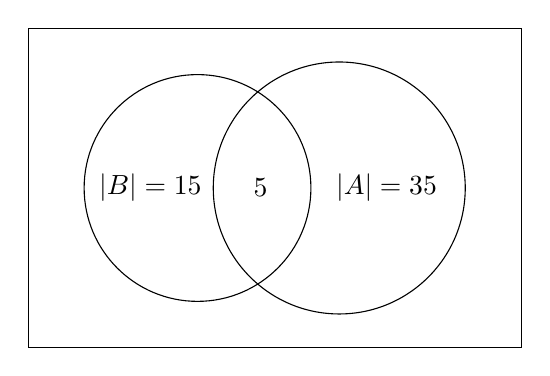
\begin{tikzpicture}[scale=.8]
		 \def\radius{2cm}
		\coordinate (ceni); 
		 \coordinate[xshift=.9*\radius] (cenii);
		\draw (ceni) circle  (.9*\radius);
		\draw (cenii) circle  (\radius);
		\draw ([xshift=-25pt,yshift=15pt]current bounding box.north west) 
			rectangle ([xshift=25pt,yshift=-15]current bounding  box.south east);
		\node[xshift=-.3*\radius] at (ceni) {$|B|=15$}; 
		\node[xshift=.3*\radius] at (cenii) {$|A|=35$}; 
		\node[xshift=.4*\radius] at  (ceni) {$5$};
	\end{tikzpicture}
	 }}
\end{bt}

% nguồn: MaHoaNH_TuLuan_Lop10
\begin{bt}%[0D1K3-3]%[ma:52894f29]
	Câu lạc bộ ngoại ngữ của trường Marie Curie có $30$ học sinh nói được  tiếng Anh, $25$ học sinh nói được tiếng Pháp, trong đó có $12$ học sinh nói được cả hai thứ tiếng Anh và Pháp. Hỏi câu lạc bộ ngoại ngữ có bao nhiêu học sinh, trong đó có bao nhiêu học sinh chỉ nói được tiếng Anh, bao nhiêu học sinh chỉ nói được tiếng Pháp?
	 \loigiai{
	 \immini
	 {
	Gọi $A$ là tập hợp ``các học sinh nói được tiếng  Anh'' thì số phần tử của $A$ là $30$.\\
	Gọi $B$ là tập hợp ``các học sinh nói được tiếng Pháp'' thì  số phần tử của $B$ là $25$.\\
	Dựa vào bổ đồ  Venn ta có
	\begin{itemize}
		\item $A\cap B$ là tập hợp các học sinh nói được cả hai thứ tiếng Anh và Pháp. Suy ra $A\cap B$ có $12$  phần tử.
		\item $A\setminus B$ là  tập hợp các học sinh chỉ nói được tiếng Anh. Suy ra $A\setminus B$ có $30-12=18$ phần tử (là số học sinh chỉ nói được tiếng Anh).
	\end{itemize}
	 }
	 {
	\begin{tikzpicture}[>=stealth]
			 \def\firstcircle{(0: 0) circle (1.2cm)}
			 \def\secondcircle{(0: 1.8) circle (1.2cm)}
			\begin{scope}
				\clip \secondcircle; 
				\fill[pattern=north east lines]  \firstcircle;
			\end{scope}
			\draw \firstcircle node[left]{$A$}; 
			\draw \secondcircle node [right]{$B$}; 
			\draw[->]  (210: 0.8)--+(-90: 1) node[below]{$A\setminus B$};
			\draw[->] (0.9,-0.2)--(0.9,-1.2)  node[below]{$A\cap B$};
			\draw[shift={(0: 1.8)},->] (-30: 0.8)--+(-90: 1)  node[below]{$B\setminus A$};
			\draw[->] (0.9,0.4)--+(90: 1.3) node[above]{$12$ Anh-Pháp}; 
			\path (100: 1.4)  node{$30$ Anh} +(0: 2.2) node{$25$ Pháp};
			\node[below] () at (0.9,-1.8){Biểu đồ Venn}; 
		\end{tikzpicture}
	 }
	\begin{itemize}
		 \item $B\setminus A$ là tập hợp các học sinh chỉ nói được tiếng Pháp. Suy ra $B\setminus A$ có $25-12=13$ phần tử (là số học sinh chỉ nói được tiếng Pháp).
		\item $A\cup B$ là  tập hợp các học sinh trong câu lạc bộ.\\
		Ta có $A\cup B=\left(A\setminus B\right)\cup \left(A\cap B\right)\cup \left(B\setminus  A\right)$.\\
		Suy ra $A\cup B$  có $18+12+13=43$ phần tử (là số học sinh trong câu lạc bộ).
	\end{itemize}
	 }
\end{bt}

% nguồn: MaHoaNH_TuLuan_Lop10
\begin{bt}%[0D1K3-3]%[ma:3a870151]
	Lớp 10X có $30$ học sinh trong đó có $25$ học sinh nói được tiếng Anh và $18$ học  sinh nói được tiếng Pháp. Hỏi có bao nhiêu học sinh nói được cả hai thứ tiếng Anh và Pháp?
	 \loigiai{
	\immini 
	 {
	Gọi $A$ là tập  hợp ``các học sinh nói được tiếng Anh'' thì số phần tử của $A$ là $25$.\\
	Gọi $B$ là tập hợp ``các học sinh nói được tiếng Pháp'' thì số phần tử của $B$  là $18$.\\
	Dựa vào bổ đồ Venn  ta có
	\begin{itemize}
		\item $A\cup B$ là tập hợp  các học sinh lớp 10X. Suy ra $A\cup B$ có $30$ phần tử.
		\item $A\setminus B$ là tập hợp  các học sinh chỉ nói được tiếng Anh.\\
		Ta có $A\setminus  B=\left(A\cup B\right)\setminus B$.\\
		Suy ra $A\setminus B$ có $30-18=12$ phần tử (là số học sinh  chỉ nói được tiếng Anh).
	\end{itemize}
	} 
	 {
	\begin{tikzpicture}[>=stealth]
			\def\firstcircle{(0:  0) circle (1.2cm)}
			\def\secondcircle{(0:  1.8) circle (1.2cm)}
			\begin{scope}
				\clip  \secondcircle;
				\fill[pattern=north  east lines] \firstcircle;
			\end{scope}
			\draw \firstcircle node[left]{$A$}; 
			\draw \secondcircle  node [right]{$B$};
			\draw[->] (210: 0.8)--+(-90: 1) node[below]{$A\setminus  B$};
			 \draw[->] (0.9,-0.2)--(0.9,-1.2) node[below]{$A\cap B$};
			\draw[shift={(0: 1.8)},->] (-30:  0.8)--+(-90: 1) node[below]{$B\setminus A$};
			\draw[->]  (0.9,0.4)--+(90: 1.3) node[above]{Anh-Pháp};
			\path (100: 1.4)  node{$25$ Anh} +(0: 2.2) node{$18$ Pháp};
			\node[below] () at  (0.9,-1.8){Biểu đồ Venn};
		\end{tikzpicture}
	 }
	\begin{itemize}
		\item $B\setminus  A$ là tập hợp các học sinh chỉ nói được tiếng Pháp.\\
		Ta có  $B\setminus A=\left(A\cup B\right)\setminus A$.\\
		Suy ra $B\setminus A$ có $30-25=5$ phần  tử (là số học sinh chỉ nói được tiếng Pháp).
		\item $A\cap B$ là tập hợp các  học sinh nói được cả hai thứ tiếng Anh và Pháp.\\
		Ta có $A\cap  B=\left(A\cup B\right)\setminus \left(\left(A\setminus B\right)\cup \left(B\setminus A\right)\right)$.\\
		Suy ra $A\cap B$ có $30-(12+5)=13$ phần tử (là số  học sinh nói được cả hai thứ tiếng Anh và Pháp).
	\end{itemize}
	} 
\end{bt}

% nguồn: MaHoaNH_TuLuan_Lop10
\begin{bt}%[0D1K3-3]%[ma:c6930384]
	Kết quả thi học kì một của một trường THPT có $48$ thí sinh giỏi môn Toán, $37$ thí sinh giỏi môn Vật Lí,$42$ thí sinh giỏi môn Văn. Biết rằng có $75$ thí sinh giỏi môn Toán hoặc môn Vật lí, $76$ thí sinh giỏi  môn Toán hoặc môn Văn, $66$ thí sinh giỏi môn Vật lí hoặc môn Văn và có $4$ thí sinh giỏi cả ba môn. Hỏi
	\begin{enumerate}
		\item có bao nhiêu học sinh chỉ giỏi  1 môn.
		\item  có bao nhiêu học sinh chỉ giỏi 2 môn.
		\item có bao nhiêu học sinh giỏi ít  nhất 1 môn.
	\end{enumerate}
	 \loigiai{
	\immini{ 
		Gọi $A$, $B$, $C$ theo thứ tự là tập hợp các học sinh giỏi Toán, giỏi Lí và giỏi Văn. Theo đề ta có 
		\begin{itemize}
			\item Số học  sinh giỏi Toán và Lí là $$|A \cap B=|A|+|B|-|A\cup B|=48+37-75=10.$$
			\item Số học sinh giỏi Toán và Văn là $$|A \cap C=|A|+|C|-|A\cup C|=48+42 - 76  = 14 .$$
			\item Số  học sinh giỏi Lí và Văn là $$|B \cap C=|B|+|C|-|B\cup C|= 42+37-66=13 .$$
			\item  Số học sinh chỉ giỏi môn Toán $48-10-6-4=28$.
			\item Số học sinh chỉ giỏi môn  Lí $37-6-4-9=18 $.
			\item Số học sinh chỉ giỏi môn Văn  $42-10-9-4=19 $.
		\end{itemize}
		}{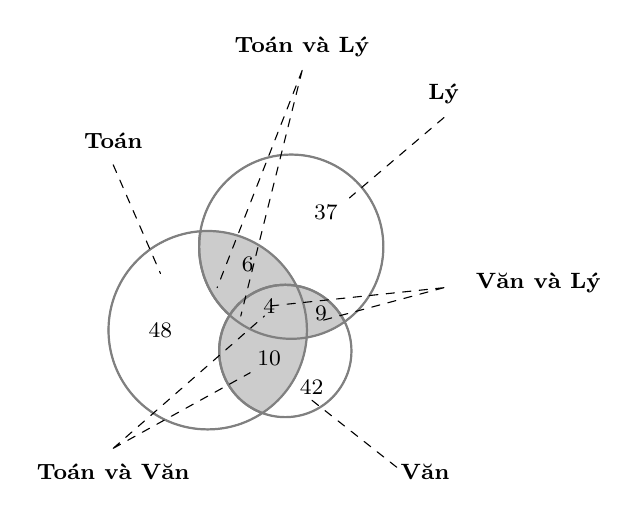
\begin{tikzpicture}[scale=0.6,>=stealth,font=\footnotesize,line join=round,line cap=round]
		\def\firstcircle{(0,0) circle  (2.1cm)}
		 \def\secondcircle{(45:2.5cm) circle (1.95cm)}
		\def\thirdcircle{(-15:1.7cm) circle (1.4cm)} 
		\colorlet{circle edge}{black!50} 
		\colorlet{circle area}{black!20} 
		\tikzset{filled/.style={fill=circle  area,draw=circle edge,thick},
			outline/.style={draw=circle edge,thick}} 
		 \draw \firstcircle;
		 \draw \secondcircle;
		\draw  \thirdcircle;
		\begin{scope}
			\clip \firstcircle; 
			 \fill[filled] \secondcircle;
		\end{scope}
		\begin{scope}
			\clip  \firstcircle;
			 \fill[filled] \thirdcircle;
		\end{scope}
		\begin{scope}
			\clip \secondcircle; 
			\fill[filled]  \thirdcircle;
		\end{scope}
		\node at (-1,0){48}; 
		\node at  (2.2,-1.2){42};
		 \node at (2.5,2.5){37};
		\node  at (0.85,1.4){6};
		\node at (1.3,0.5){4}; 
		\node  at (1.3,-0.6){10};
		 \node at (2.4,0.35){9};
		 \draw[outline] \firstcircle
		 \secondcircle \thirdcircle;
		\node at (-2,4)  {\textbf{Toán}};
		\node at (2,6) {\textbf{Toán và Lý}}; 
		\node at (5,5) {\textbf{Lý}}; 
		\node at (7,1) {\textbf{Văn và Lý}}; 
		 \node at (4.6,-3) {\textbf{Văn}};
		\node  at (-2,-3) {\textbf{Toán và Văn}};
		\draw[dashed]  (-2,3.5) -- (-1,1.2)
			 (2,5.5) -- (0.7,0.3)
			 (2,5.5) -- (0.2,0.9)
			 (5,4.5) -- (3,2.8)
			(5,0.9) -- (1.2,0.5) 
			(5,0.9)  -- (2.4,0.2)
			(4,-2.9) --  (2.1,-1.4)
			(-2,-2.5)  -- (1.2,0.3)
			 (-2,-2.5) -- (0.9,-0.9);
	\end{tikzpicture}
		 }
		\begin{enumerate}
			\item Số học sinh chỉ  giỏi đúng 1 môn là $28+18+19=65$.
			\item Số học sinh chỉ giỏi đúng  2 môn là $10+6+9=25$.
			\item Số học sinh giỏi ít nhất một môn là  $65+25+4=94$.
		\end{enumerate}
	 }
\end{bt}
